\subsection{Interrelación Plantilla Entrevista Asesor - Pregunta Asesor}

   \begin{description}
      \item[Definición] En esta interrelación se deja constancia de que una
      plantilla de entrevista de asesor puede estar compuesta por varias
      preguntas de asesor.

      \begin{itemize}
       \item Una \textit{Plantilla Entrevista Asesor} puede contener varias
             \textit{Pregunta Asesor}.
       \item Una \textit{Pregunta Asesor} solamente puede formar parte de una
             \textit{Plantilla Entrevista Asesor}.
      \end{itemize}

      \item[Características] La interrelación presenta las siguientes
                             características:

         \begin{itemize}
            \item \textbf{Nombre:} PEA-PA
            \item \textbf{Tipo de la interrelación:} El tipo de entidad Pregunta
                  Asesor es débil por identificación respecto al tipo de
                  entidad Plantilla Entrevista Asesor.
            \item \textbf{Cardinalidad de la interrelación:} 1:N
                  \begin{itemize}
                     \item Plantilla Entrevista Asesor: contiene (0,n)
                     \item Pregunta Asesor: forma\_parte\_de (1,1)
                  \end{itemize}
            \item \textbf{Número de atributos:} Ninguno.
         \end{itemize}

      \item[Diagrama] La figura \ref{diagramaPEA-PA} muestra el diagrama de la
                      interrelación.

      \item \begin{figure}[!ht]
            \begin{center}
            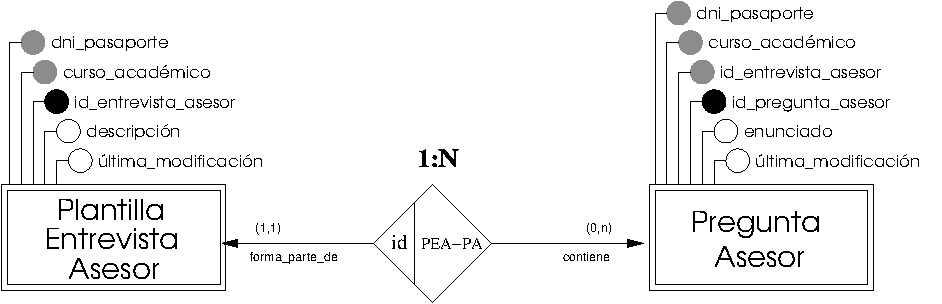
\includegraphics[]{07.Modelo_Entidad-Interrelacion/7.3.Analisis_Interrelaciones/diagramas/PEA-PA.pdf}
            \caption{Diagrama de la interrelación PEA-PA.}
            \label{diagramaPEA-PA}
            \end{center}
         \end{figure}

      \item[Ejemplo práctico del tipo de interrelación]

      \item \begin{center}
            \begin{tabular}{ | r r | }
            \hline
            \multicolumn{2}{ | c | }{\textbf{Tipo de interrelación PEA-PA}} \\
            \hline
            \textbf{Plantilla Entrevista Asesor} & \\
            dni\_pasaporte & 98765432Z \\
            curso\_académico & 2008 \\
            id\_entrevista\_asesor & 36 \\
            \hline
            \textbf{Pregunta Asesor} & \\
            dni\_pasaporte & 98765432Z \\
            curso\_académico & 2008 \\
            id\_entrevista\_asesor & 36 \\
            id\_pregunta\_asesor & 72 \\
            \hline
            \end{tabular}
         \end{center}
   \end{description}
